\documentclass[12pt]{article}
\usepackage[utf8]{inputenc}
\usepackage[english]{babel}
\usepackage[backend=biber,style=numeric,sorting=ynt]{biblatex}
\usepackage{url}
\usepackage{longtable}
\usepackage{amsmath}
\usepackage{graphicx}
\graphicspath{{figures/}}
\usepackage{parskip}
\usepackage{fancyhdr}
\usepackage{vmargin}
\usepackage{float}
\usepackage{verbatim}
\usepackage{multicol}
\usepackage{xspace}
\setmarginsrb{3 cm}{2.5 cm}{3 cm}{2.5 cm}{1 cm}{1.5 cm}{1 cm}{1.5 cm}
\addbibresource{ref.bib}

%%% EDIT THIS INFORMATION TO MAKE RELEVANT UPDATES FOR YOUR SPECIFIC REPORT%%%
%%%↓↓↓↓↓↓↓↓↓↓↓↓↓↓↓↓↓↓↓↓↓↓↓↓↓↓↓↓↓↓↓↓↓↓↓↓↓↓↓↓↓↓↓↓↓↓↓↓↓↓↓↓↓↓↓↓↓↓↓↓↓↓↓↓↓↓↓↓%%%
\newcommand{\reportName}{Lab 1\xspace}
\newcommand{\reportTopic}{Helicopter Control\xspace}
\newcommand{\courseName}{EEE3094S\xspace}
\newcommand{\courseTitle}{Control Systems Engineering\xspace}
\newcommand{\authorFullName}{Matekoa Motsoasele\xspace}
\newcommand{\authorStudentNumber}{MTSMAT027\xspace}
\newcommand{\dueDate}{01 October 2021\xspace}
%%%↑↑↑↑↑↑↑↑↑↑↑↑↑↑↑↑↑↑↑↑↑↑↑↑↑↑↑↑↑↑↑↑↑↑↑↑↑↑↑↑↑↑↑↑↑↑↑↑↑↑↑↑↑↑↑↑↑↑↑↑↑↑↑↑↑↑↑↑%%%

\title{\reportName - \reportTopic}	% Title
\author{\authorFullName (\authorStudentNumber)}	% Author
\date{\today}									% Date

\makeatletter
\let\thetitle\@title
\let\theauthor\@author
\let\thedate\@date
\makeatother

\pagestyle{fancy}
\fancyhf{}
\rhead{\theauthor}
\lhead{\thetitle}
\cfoot{\thepage}



\begin{document}

%%%%%%%%%%%%%%%%%%%%%%%%%%%%%%%%%%%%%%%%%%%%%%%%%%%%%%%%%%%%%%%%%%%%%%%%%%%%%%%%%%%%%%%%%

\begin{titlepage}
	\centering
    \vspace*{0.5 cm}
    
\includegraphics[scale = 0.75]{UCT.jpg}\\[1.0 cm]	% University Logo
    \textsc{\LARGE University of Cape Town}\\[2.0 cm]	% University Name
	\textsc{\Large \courseName}\\[0.5 cm]				% Course Code
	\textsc{\large \courseTitle}\\[0.5 cm]	% Course Name
	\rule{\linewidth}{0.2 mm} \\[0.4 cm]
	{ \huge \bfseries \thetitle}\\
	\rule{\linewidth}{0.2 mm} \\[1.5 cm]
	
	\begin{minipage}{0.4\textwidth}
		\begin{flushleft} \large
			\emph{Report Author:}
			\end{flushleft}
			\end{minipage}~
			\begin{minipage}{0.4\textwidth}
			\begin{flushright} \large
			\emph{\theauthor} \\
		\end{flushright}
	\end{minipage}\\[4 cm]
	
	{\large Due: \dueDate}\\[2 cm]
 
	\vfill
	
\end{titlepage}

%%%%%%%%%%%%%%%%%%%%%%%%%%%%%%%%%%%%%%%%%%%%%%%%%%%%%%%%%%%%%%%%%%%%%%%%%%%%%%%%%%%%%%%%%

\tableofcontents
\pagebreak

%%%%%%%%%%%%%%%%%%%%%%%%%%%%%%%%%%%%%%%%%%%%%%%%%%%%%%%%%%%%%%%%%%%%%%%%%%%%%%%%%%%%%%%%%

\section{\Large{Introduction}}

The aim of the lab is to identify the system parameters/model given a helicopter model with commanded blade angle of attack as an input and height as an output.

Using a blackbox model, we are able to develop a model of the system from the measured data and a transfer function is found using various methods. 
\\\\
%%%%%%%%%%%%%%%%%%%%%%%%%%%%%%%%%%%%%%%%%%%%%%%%%%%%%%%%%%%%%%%%%%%%%%%%%%%%%%%%%%%%%%%%%

\section{\Large{Model Development}}

Figure 1 shows the Mathematical model of the helicopter. The System dynamics are unknown and so a black box model approach must be used to find the parameters of the model.\cite{2} The pitch angle can be interpreted as a voltage by use of a potentiometer, this way, the input can be taken as a voltage. 

 \begin{figure}[H]
     \centering
     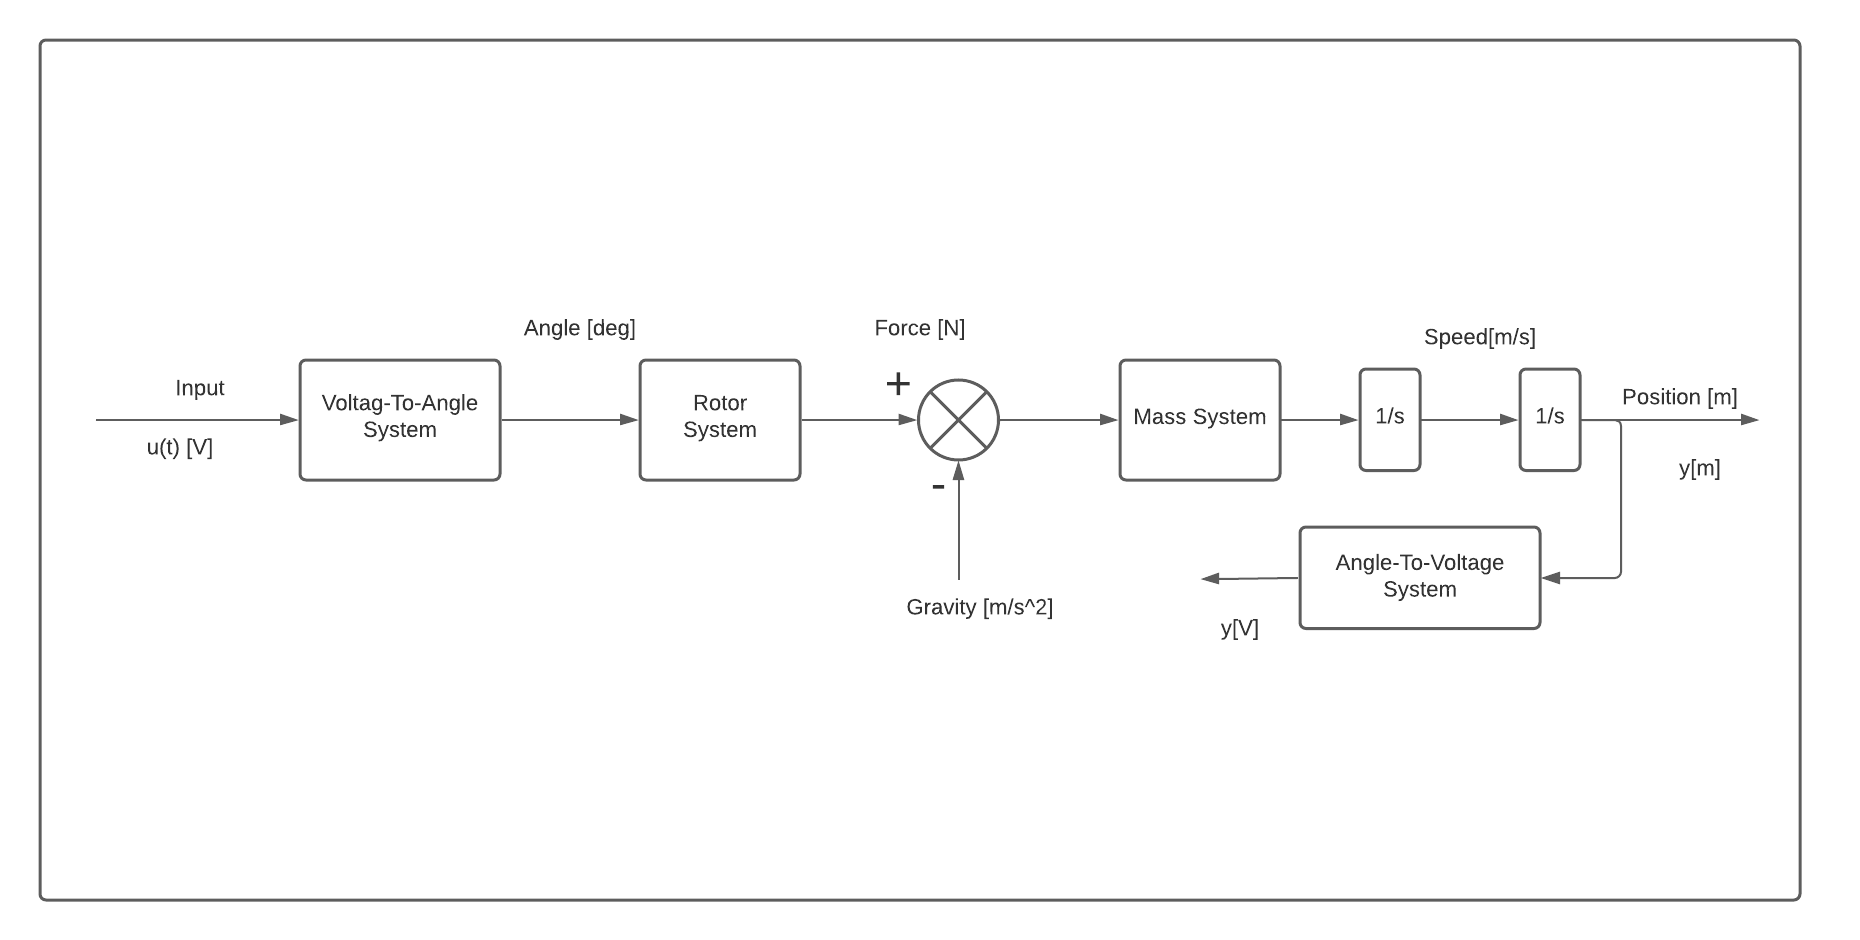
\includegraphics[width=0.9\textwidth]{model.png}
     \caption{Helicopter Mathematical Model}
     \label{fig:sample}
 \end{figure}



%%%%%%%%%%%%%%%%%%%%%%%%%%%%%%%%%%%%%%%%%%%%%%%%%%%%%%%%%%%%%%%%%%%%%%%%%%%%%%%%%%%%%%%%%

% \begin{figure}[H]
%     \centering
%     \includegraphics[width=0.75\textwidth]{sample.png}
%     \caption{Sample Caption}
%     \label{fig:sample}
% \end{figure}

\newpage

\section{\Large{System Identification}}
To identify system parameters, two methods were used and compared. The approach in system identification was that of a black box model because the only information that was available was the input and the output. The objective here is to find the transfer function G(s). 
\begin{figure}[H]
     \centering
     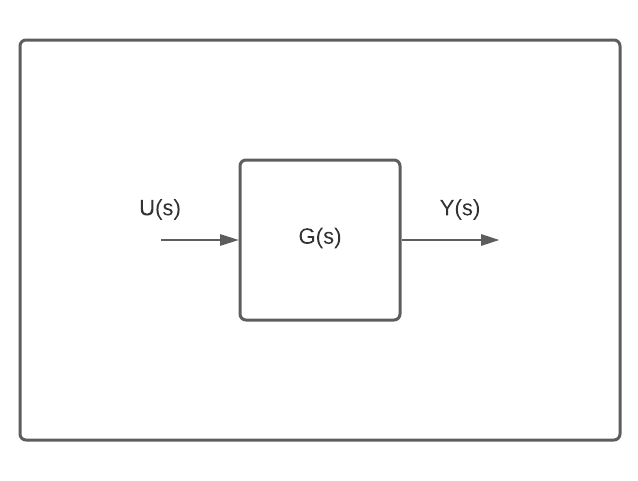
\includegraphics[width=0.4\textwidth]{transfer.png}
     \caption{Simplified Block Diagram}
     \label{fig:sample}
 \end{figure}



\subsection{\Large{Hand Method}}

The measured input step is shown below

From the measured data, the step response is plotted in the time domain where the output is the speed. 

\begin{figure}[H]
     \centering
     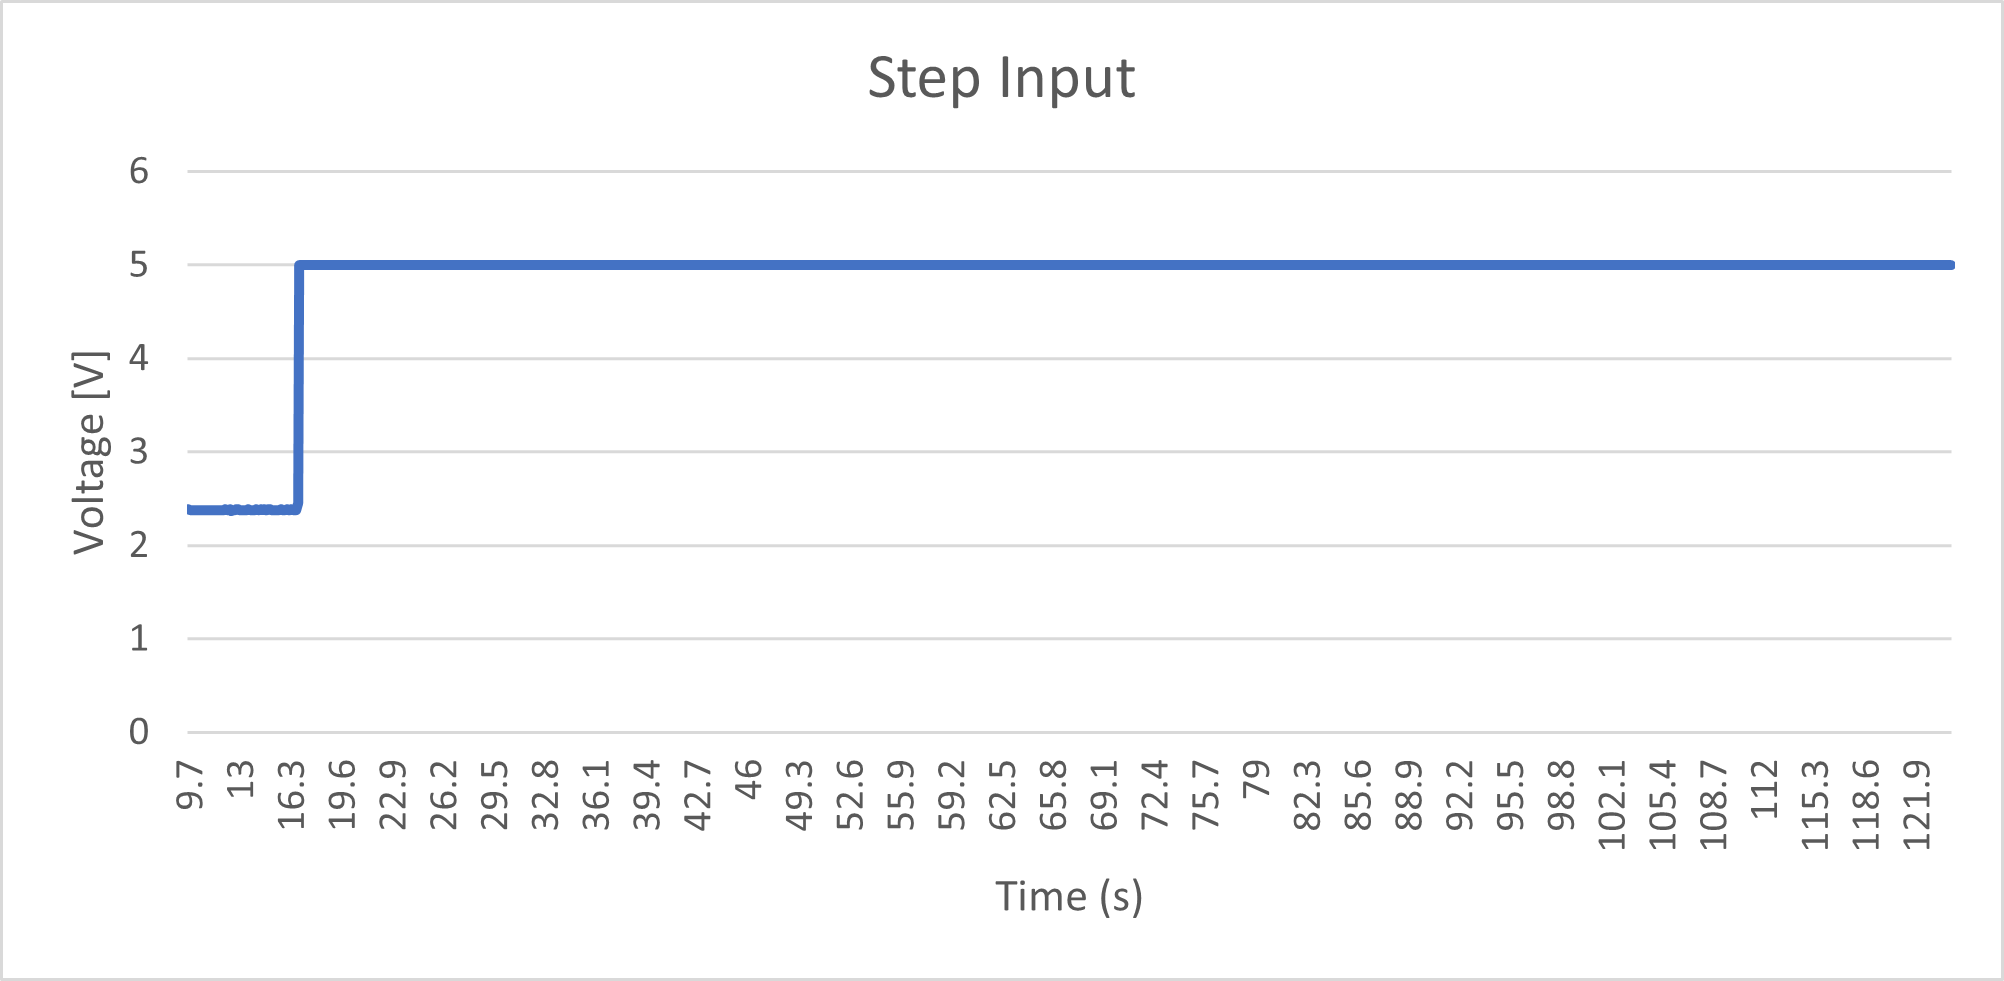
\includegraphics[width=0.5\textwidth]{inputstep.png}
     \caption{Step Input}
     \label{fig:sample}
 \end{figure}
 The input is given by:
\[
    Input = B*u(s)
\]
where B is the size of the step.

The Laplace transform of the step input is given by:

\[ U(s) = \frac{B}{s} \]

 By taking an instantaneous change in displacement we are able to obtain the speed as shown in Figure 4.
 \begin{figure}[H]
     \centering
     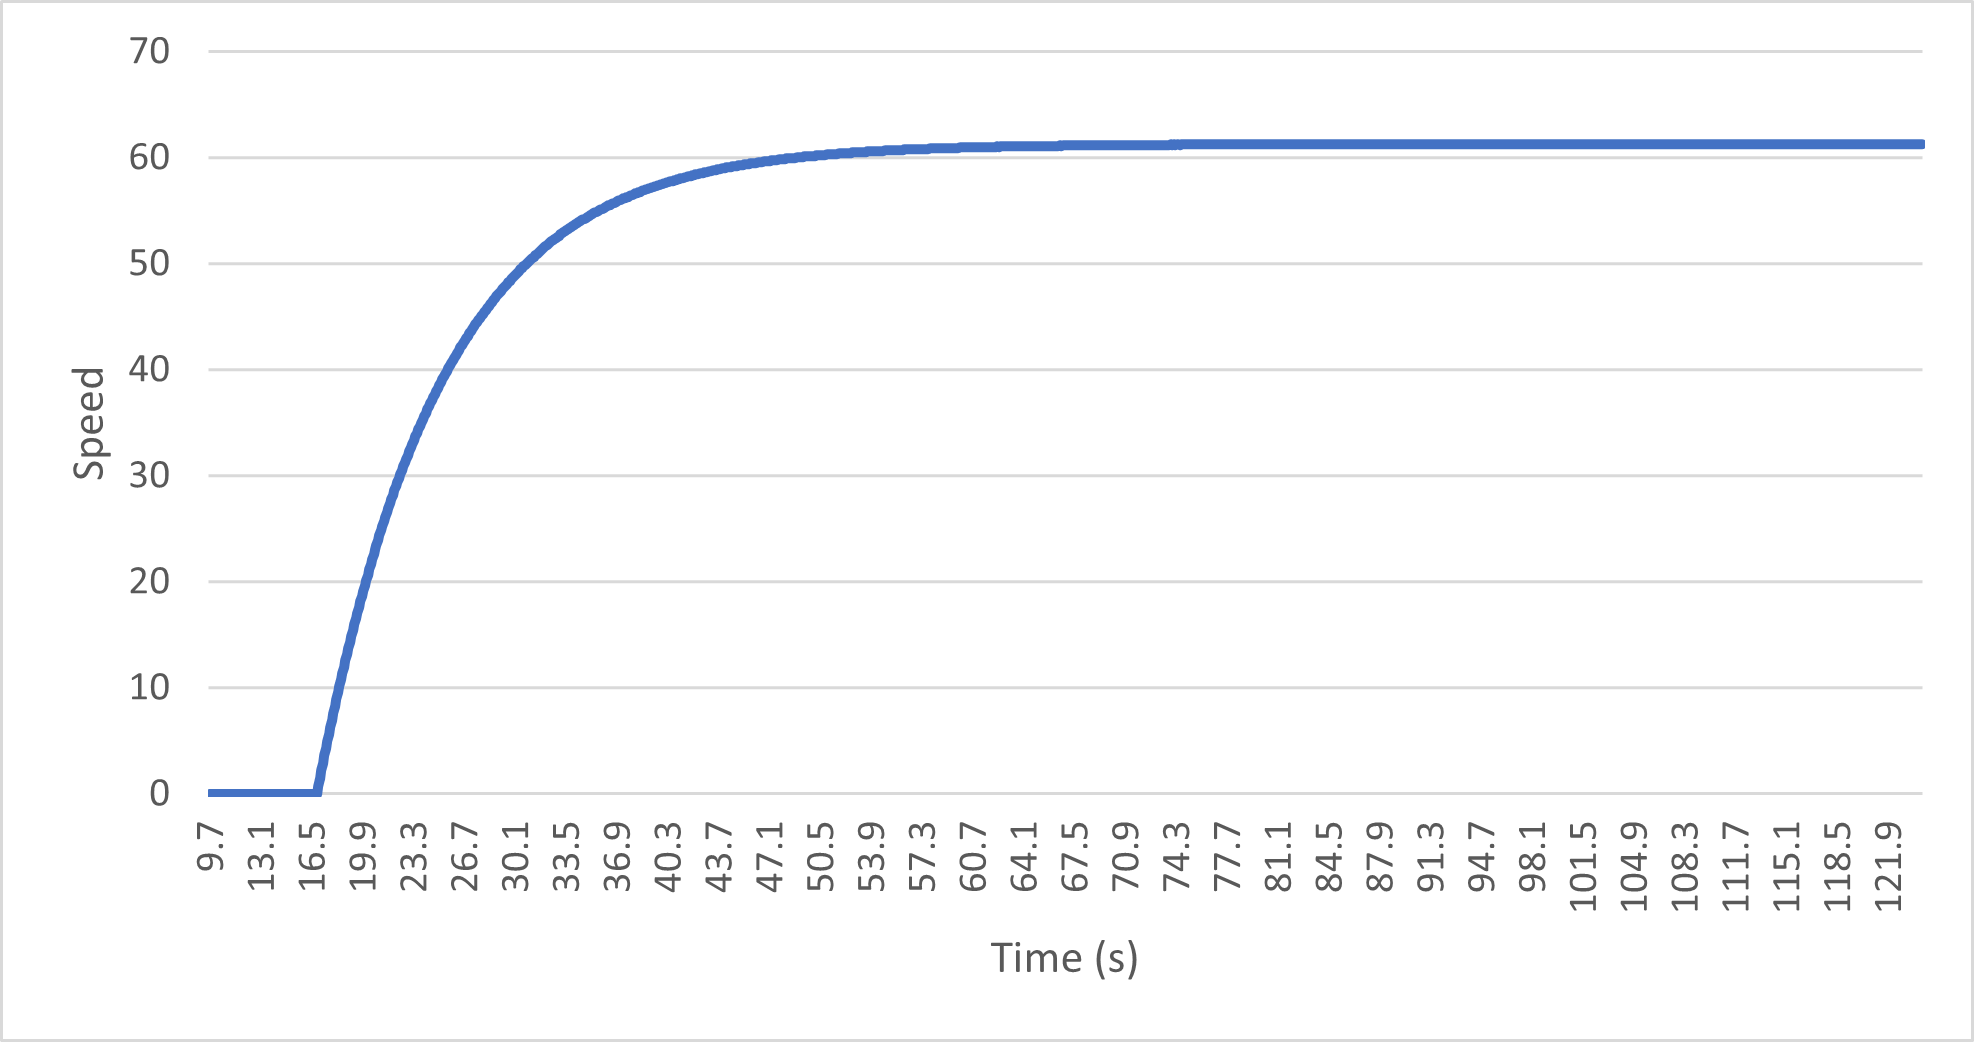
\includegraphics[width=0.5\textwidth]{outputmeas.png}
     \caption{Step Response in Time Domain}
     \label{fig:sample}
 \end{figure}
 
 This gives us the step response in the time domain which is represented by:
 
 \[
    y(t) = AB(1-e^{\frac{-t}{\tau}})
 \]
 In this form, the time constant can be found as a value of time that occurs at around 63\% of the steady state speed.\\
 
 The terminal velocity of the helicopter is the speed at steady state. This is given by:

\[ v_t = AB = 61.275 m/s \]

 The transfer function of this system can be expressed in the general form:

\[ G(s) = \frac{A}{(1+s\tau)} \]

The step response in the Laplace domain then becomes:

\[
    Y(s) = \frac{AB}{s(1+\tau s)}
\]
Where A is the gain and \( \tau \) is the time constant.

The value of s is given by:

\[ s = V/m = 0.7 \]

where V is the input voltage and m is the height in meters.

Using this method, the approximate values are found to be:

\[
    A = 24.51
\]
\[
    \tau = 8.32 seconds
\]

% \begin{figure}[H]
%     \centering
%     \includegraphics[width=0.75\textwidth]{sample.png}
%     \caption{Sample Caption}
%     \label{fig:sample}
% \end{figure}



\subsection{\Large{System Identification Toolbox}}
To obtain the transfer function via simulation, the System Identification Toolbox in MATLAB was used. Before the input voltage data can be used, 2.5V is subtracted as this is the hovering voltage characteristic of the helicopter. The output is picked to be speed, which is the \( \frac{\Delta h}{\Delta t} \) This allows us to represent the transfer function as a first order function with 1 pole. The input and output data are shown in the figure below.

\begin{figure}[H]
     \centering
     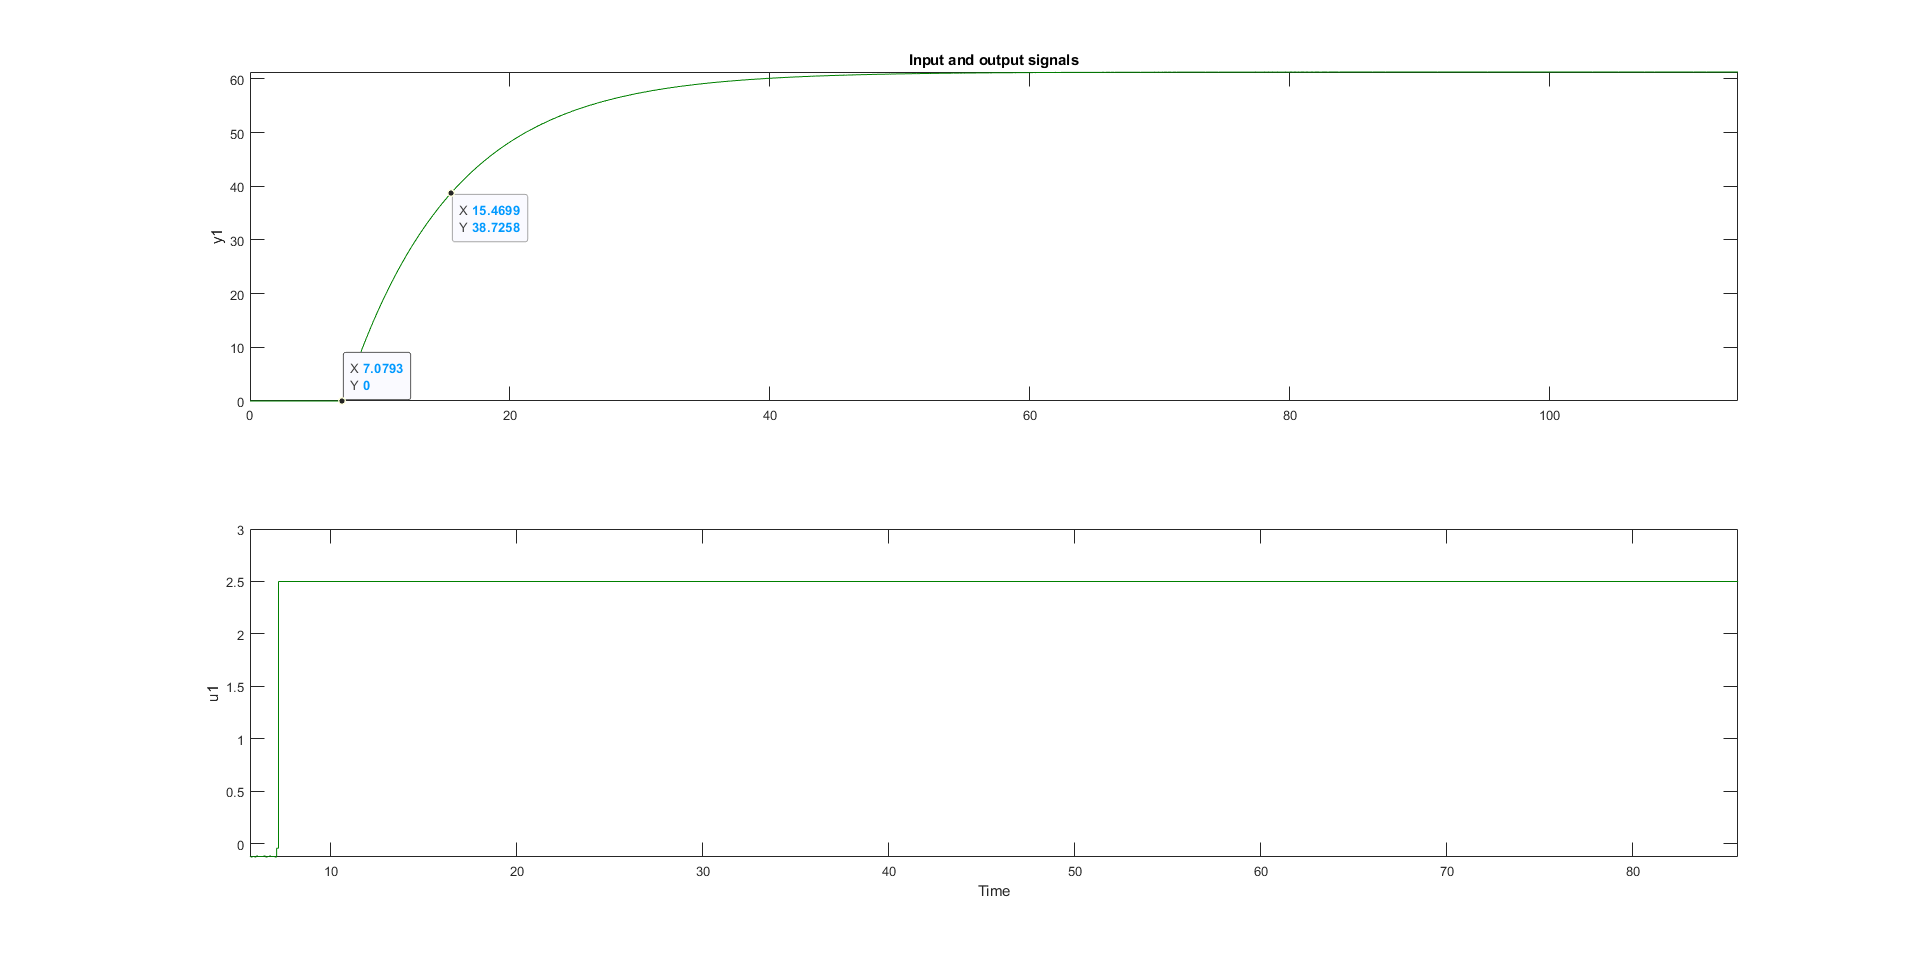
\includegraphics[width=0.75\textwidth]{inputvsoutput.png}
     \caption{Imported Input and Output Data Plots}
     \label{fig:sample}
 \end{figure}

From the data, the following transfer function is obtained:
\[
    G(s) = \frac{3.017}{s+0.1232}
\]
By dividing by the constant in the denominator, the form \( G(s) = \frac{A}{1+ \tau s} \) is obtained to be:
\[
    G(s) = \frac{24.35}{8.12s+1}
\]

The step response Y(s) in the Laplace Domain is given by:
\[
    Y(s) = U(s)G(s)
\]
\[
    Y(s) = \frac{24.35}{s(8.12s+1)}
\]
The value of A is the gain and can be shown by the step response plot below.
\begin{figure}[H]
     \centering
     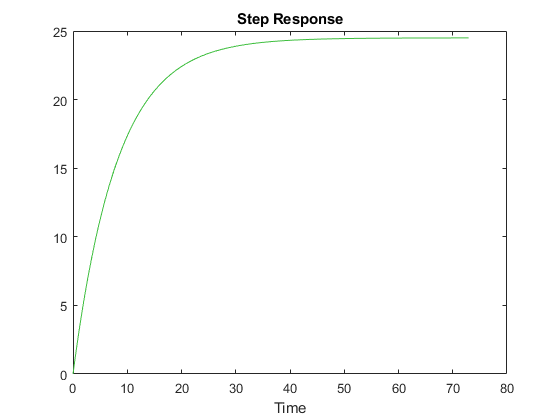
\includegraphics[width=0.5\textwidth]{step response.png}
     \caption{System Identification Step Response}
     \label{fig:sample}
 \end{figure}
Using System Identification Toolbox, the parameters are as follows: \\
A = 24.35 \\
\(\tau \) = 8.12 seconds
\newpage

%%%%%%%%%%%%%%%%%%%%%%%%%%%%%%%%%%%%%%%%%%%%%%%%%%%%%%%%%%%%%%%%%%%%%%%%%%%%%%%%%%%%%%%%%


%%%%%%%%%%%%%%%%%%%%%%%%%%%%%%%%%%%%%%%%%%%%%%%%%%%%%%%%%%%%%%%%%%%%%%%%%%%%%%%%%%%%%%%%%

\section{\Large{Analysis, interpretation and discussion}}
Figure compares the step responses from the hand method and System Identification. Through this, it is evident that the step responses are very similar. tf1 in the chart represents the transfer function from the hand method, while tf5 represents the transfer function obtained from the system identification toolbox.
\begin{figure}[H]
     \centering
     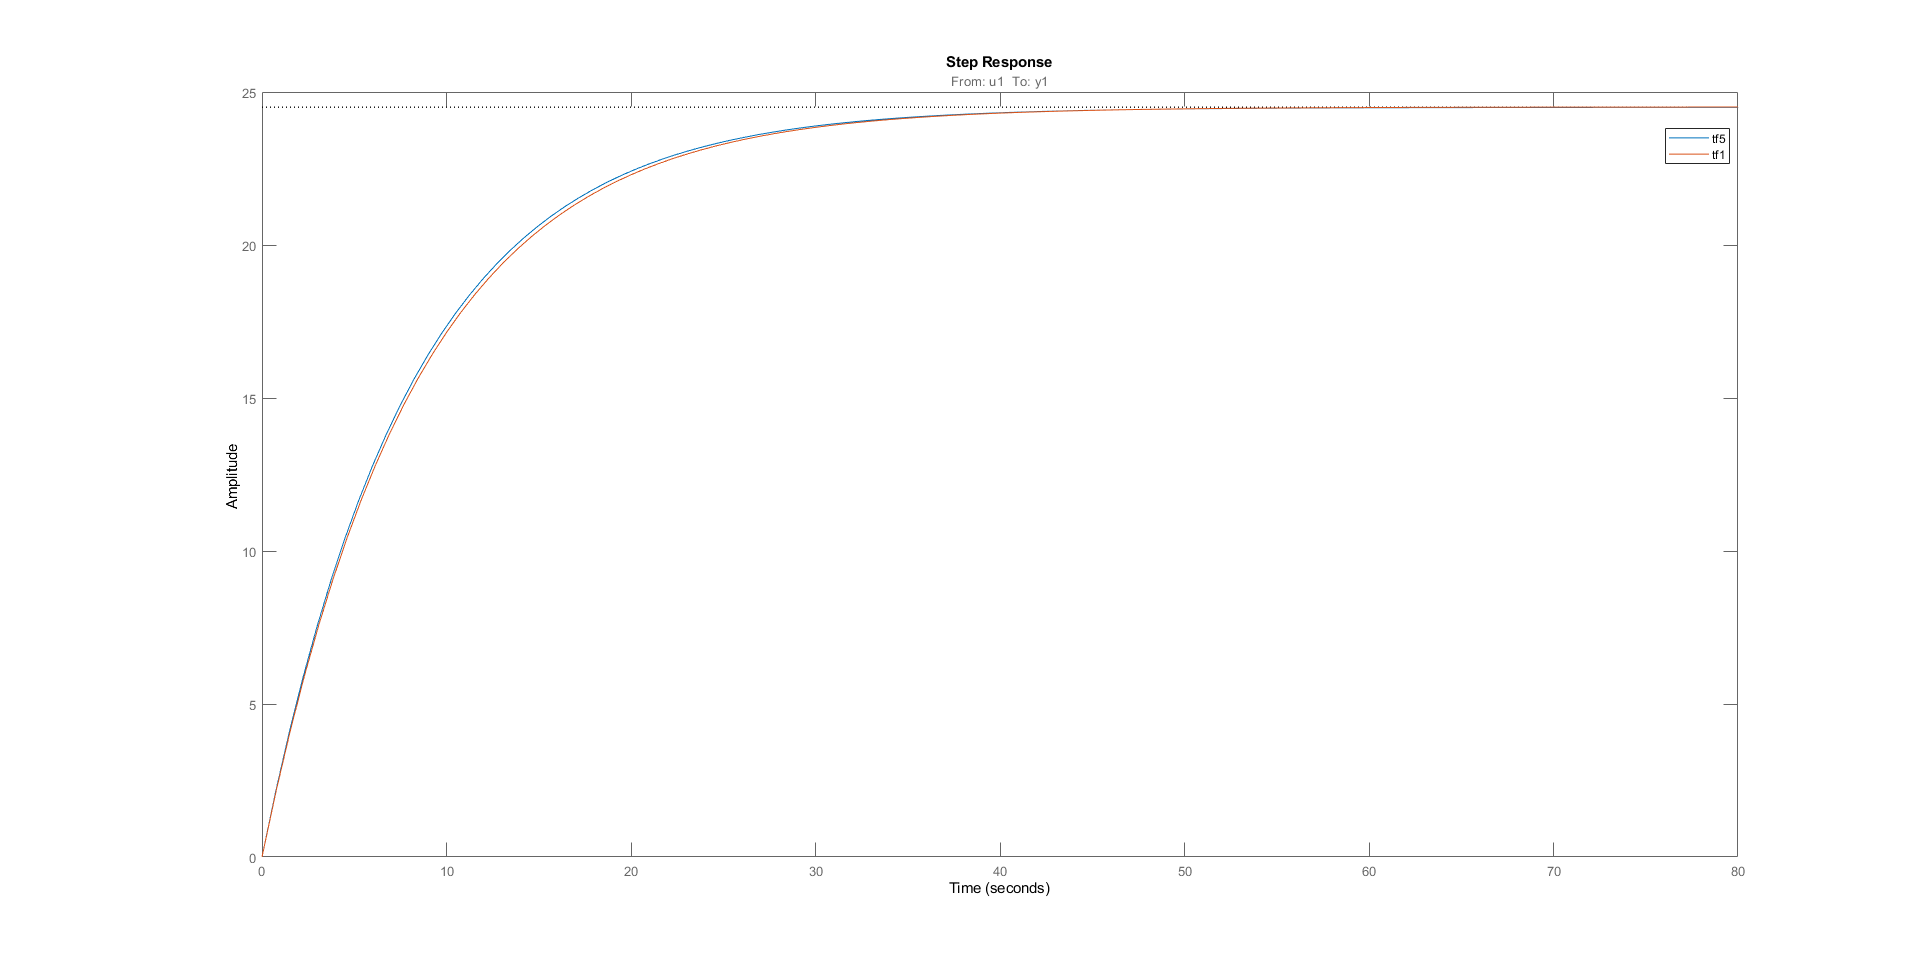
\includegraphics[width=0.7\textwidth]{step response comparison.png}
     \caption{Step Response Comparisons}
     \label{fig:sample}
 \end{figure}

"A" from system identification Toolbox compared to "A" from the hand method is 99.3\% accurate.\\

Comparing the time constants from System Identification Toolbox and the Hand method gives us 97\% accuracy between the two values.

\newpage

%%%%%%%%%%%%%%%%%%%%%%%%%%%%%%%%%%%%%%%%%%%%%%%%%%%%%%%%%%%%%%%%%%%%%%%%%%%%%%%%%%%%%%%%%

\section{\Large{Conclusions}}

A black box approach was used in the system identification to determine the transfer function of the helicopter model. Two methods were used and compared. The values of the two approaches were compared. From system Identification the parameters obtained were A = 24.35 and the time constant \( \tau \)= 8.12 seconds. Using the hand method, the values obtained were A = 24.51, \( \tau \) = 8.32 seconds and the sensor value was 0.7 [V/m].
\newpage

%%%%%%%%%%%%%%%%%%%%%%%%%%%%%%%%%%%%%%%%%%%%%%%%%%%%%%%%%%%%%%%%%%%%%%%%%%%%%%%%%%%%%%%%%

\section{\Large{References}}
\nocite{*}
\printbibliography

%%%%%%%%%%%%%%%%%%%%%%%%%%%%%%%%%%%%%%%%%%%%%%%%%%%%%%%%%%%%%%%%%%%%%%%%%%%%%%%%%%%%%%%%%
\end{document}